\documentclass[11pt]{article}
\usepackage{geometry, amssymb, marvosym, enumitem, mathtools,amsthm, tikz, float}
\geometry{margin = 1in}
\linespread{1.25}
\usepackage[utf8]{inputenc}
\title{Manuscript}
\author{}
\date{September 2020}
\newcommand{\LL}[1]{{\textcolor{magenta}{\small {\sf [[LL: #1]]}}}}
\newcommand{\x}[0]{\mathbf{x}}
\begin{document}

\maketitle
\begin{abstract}
    This work provides an empirical study of the computational cost and effectiveness of several common optimization procedures applied to homological generators in dimension one, including algorithms to minimize $L_0$ and $L_1$ norms, bounding area, and “volume.” We conduct these optimizations via standard linear programming methods, applying general-purpose solvers to optimize over column bases of simplicial boundary matrices. Our key findings are (i) the computational cost of optimizing a basis of generators exceeds the cost of computing such a basis, for each of the tested general-purpose solvers, (ii) optimization is generally effective in reducing the size of generators, though the extent of the reduction varies according to the distribution of the underlying data, and (iii)  the space of $L_1$ optimal solutions properly contains that of $L_0$ optimal solutions in the majority of Vietoris-Rips complex studied, though none of these complexes had totally-unimodular boundary matrices in degree one, a sufficient condition found in other studies.
\end{abstract}

\textcolor{red}{
Last week:\\
1. Found inefficiency in computeHomology pipeline and sped up the process \\
2. Ran experiments on roadmap datasets. \\
3. Confirmed that the optimum cost found by using basis columns and full columns are the same.\\
4. Using basis columns may introduce machine error but should give the same solution if we round. }

% 1. try basis columns to put into gurobi; \\
% 2. explore relationship between the length of time to compute vs size of the bdr matrix \\
% 3. Add a plot for number of generators and generator size for different distributions and dimensions \\
% 4. Compare GLPK and Gurobi and report statistics\\
\section{Introduction}

Approaches to minimal generators \cite{Escolar2016,Dey2019,Obayashi2018}. 


\section{Related Work}

Barcodes \cite{Ghrist08}\\
Lori Chad Tom \cite{TZH15}\\
Eirene \cite{henselman2016matroid}\\
Escolar Optimal Cycles \cite{Escolar2016}\\
Obayashi Volume-Optimal Cycles \cite{Obayashi2018}\\
Dey Optimal 1-cycles \cite{Dey2019}\\
Roadmap \cite{roadmap2017}\\

\section{Problem formulation}
% This subsection is meant to serve as a brief description of \cite{Escolar2016}. Refer to the original paper for more thorough descriptions (including pseudo code) or details regarding computational complexity. Suppose we have a $q$-cycle $z$ which we seek to minimize with respect to the 1 norm $\left|\left| \sum a_j\sigma_j \right|\right| = \sum |a_j|$ on the space $C_q(K) = \text{span}\{\sigma_j\}$, where $\sigma_j$ are $q$ simplices in $K$. A first approach to minimization could be to consider the linear optimization problem
\begin{align*}
    \text{minimize } & ||x||_1\\
    \text{subject to } & x - \partial_{q+1}y = z\\
    & x, y \text{ integral}
\end{align*}
where $\partial_{q+1}$ is the $q+1$st boundary matrix and $y$ is any $q+1$-chain. Essentially, this system of equations searches for a $q$-chain $x$ with minimal size which is homologous to our original cycle $z$. We call our minimal solution $x = \Tilde{z}$. Now instead, suppose we have a simplex-wise filtration $K_b$, where one simplex $\sigma_b$ is added at each filtration step. At any given filtration step, then, we gain at most one $q$-cycle. Call that $q$-cycle $z$ and call previous (known) cycles $\{g_j\}$ and consider the following problem, modified from above:
\begin{align*}
    \text{minimize } & ||x||_1\\
    \text{subject to } & x - \partial_{q + 1}y + \sum a_j g_j = z\\
    & x,y,a \text{ integral}
\end{align*}
We call our solution to this algorithm $\Tilde{z}_j$. Finally, if we let $\{\Tilde{z}_j\} = \{g_j\}$ be minimal cycles found at previous steps and perform the above algorithm, we find a minimal cycle at each step.

One observation regarding this algorithm is that it computes an optimal cycle $\Tilde{z}_j$ only once, then does not modify it. If, for example, the feature enclosed by $\Tilde{z}_j$ split into two holes, $\Tilde{z}_j$ would enclose both holes. Although this might not be considered ``optimal" at this step, modifying $\Tilde{z}_j$ at future steps would likely produce a cycle that does not exist for the entire time the feature persists.


Below is an example of the result of this algorithm, sampled from a noisy circle:
\begin{figure}[h]
    \centering
    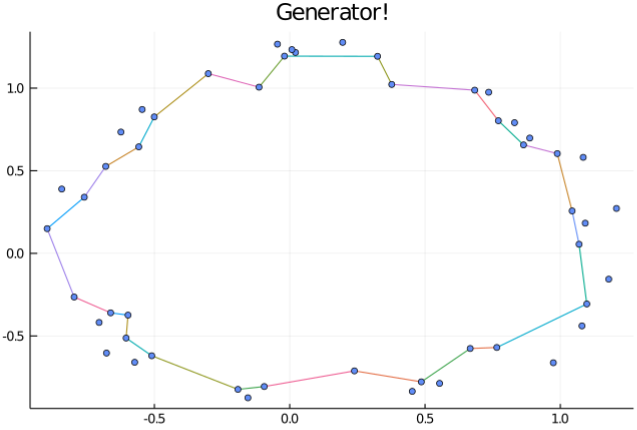
\includegraphics[width = .45\textwidth]{NoisyCircleOrig.png}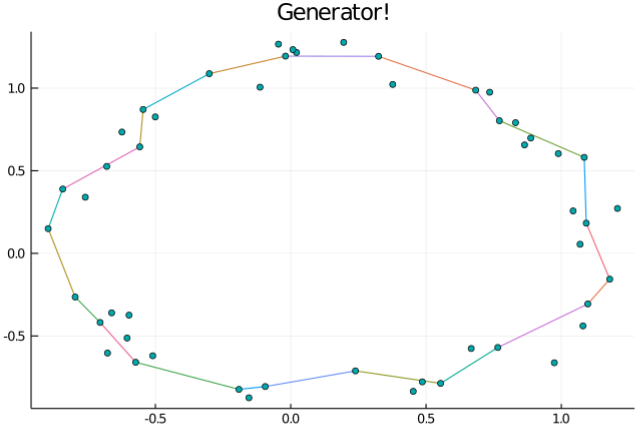
\includegraphics[width = .45\textwidth]{NoisyCircleMin.png}
    \caption{A generator found from our algorithm (left) and the minimal version of it (right) found via linear programming as described in \cite{Escolar2016}}
    \label{EscolarMinGen}
\end{figure}
Note this cycle is not also volume-minimal: the original generator contains 28 1-simplices, and the minimal version contains 21, but the minimal version encloses a greater area. See a later section and \cite{Obayashi2018} for an algorithm which computes volume-optimal cycles. Also note that some modifications to the generator were unnecessary: around the (-.5,.75) coordinate the generator switches between one pair of 1-simplices and another, for no clear reason.





Given an integer valued $1$-chain $c = \sum_{i=0}^{m-1} a_i \sigma_i$, we use $\mathbf{x} \in \mathbb{Z}^m$ to denote the vector formed by the coefficients $a_i.$ 
For a vector $\mathbf{v} \in \mathbb{R}^m$, the $1-norm$ (or $\ell^1-$norm) $||\mathbf{v}||_1$ is defined to be $\sum_i|v_i|.$ Let $\mathbf{w} \in \mathbb{R}^m$. Then, the $1$-norm of the dot product of $\mathbf{w} $ and $\mathbf{v}$, that is, $||\mathbf{w}\cdot \mathbf{v}||_1$ is $\sum_i|w_i||v_i|.$ 

Given a $1$-chain $c$ and a weight vector $\mathbf{w}$, we use linear programming to find a chain $c^*$ which has the minimal $1$-norm $||\mathbf{w} \cdot  \mathbf{x^*}||_1$ among all chains homologous to $c.$

Our problem is therefore weighted $\ell^1-$optimization of homologous chains. We can achieve different types of optimality by choosing different weight for the simplices. For example, suppose we have $\mathbf{w} \in \mathbb{R}^n$ such that $w_i$ equal to the length of the $\sigma_i$. Then, the resulting optimal chain has the smallest length among all chains homologous to $c.$ If $\mathbf{w}$ is taken to be $\mathbf{1},$ then we are assigning uniform weights to each simplex in $c.$ Then, the resulting optimal chain has the smallest number of simplices among all chains homologous to $c.$

In addition to varying the weight of each simplex, we can also choose between doing linear programming or integer linear programming. If we require an integer solution and the resulting $\mathbf{x}$ has all entries in $\{-1,0,1\},$ then we can solve the $\ell^0$-optimization problem. 

Combining the algorithms discussed above, we experimented solving the weighted $\ell^1$-optimization problem, with four different constraints: 

$$\text{min} ||\mathbf{w} \cdot \mathbf{x}||_1 \text{ subject to: } \\ \mathbf{x} - \partial_{2} \mathbf{y} + \sum a_jg_j = c $$
\begin{enumerate}
    \item[i.] $\mathbf{w} = \mathbf{1}.$
    \item[ii.] $\mathbf{w}$ where $w_i = len(\sigma_i).$
    \item[iii.] $\mathbf{w} = \mathbf{1},$ $\mathbf{x}, \mathbf{y}, a$ integral. 
    \item[iv.]  $\mathbf{w}$ where $w_i = len(\sigma_i)$ , $\mathbf{w} = \mathbf{1},$ $\mathbf{x}, \mathbf{y}, a$ integral. 
\end{enumerate}

\section{Experiments}

\subsection{Data}
\begin{enumerate}
    \item We perform experiments on $450$ data sets, each containing $100$ points in $R^n$ with $n$ from $2$ to $10,$ randomly drawn from the following  continuous distributions: Normal, Exponential,  Logarithmic. We randomly sample $10$ data sets for each distribution and dimension pair. 
    \item Real world data sets:
    \begin{enumerate}
        \item Vicsek biological aggregation model. $3 \times 300.$ Computation time: $206.35$ seconds. 
        \item Klein bottle in $3$-D $3\times 400$.   $13216$ seconds ($\approx 3.6$ hours)
        \item Random VR complexes (uniform distribution) $16\times 50$. $0.82$ seconds.
        \item 
    \end{enumerate}
\end{enumerate}


\subsection{Linear Programming Solvers}
In the original paper \cite{Escolar2016}, the authors implemented this linear programming algorithm using the GLPK(GNU Linear Programming Kit) linear solver. 
Our experiments show that the solvers used in these optimizing algorithms could greatly impact: 1. the computation time 2. the optimal solutions. \\

\begin{figure}[h]
\begin{minipage}[b]{3.5in}
    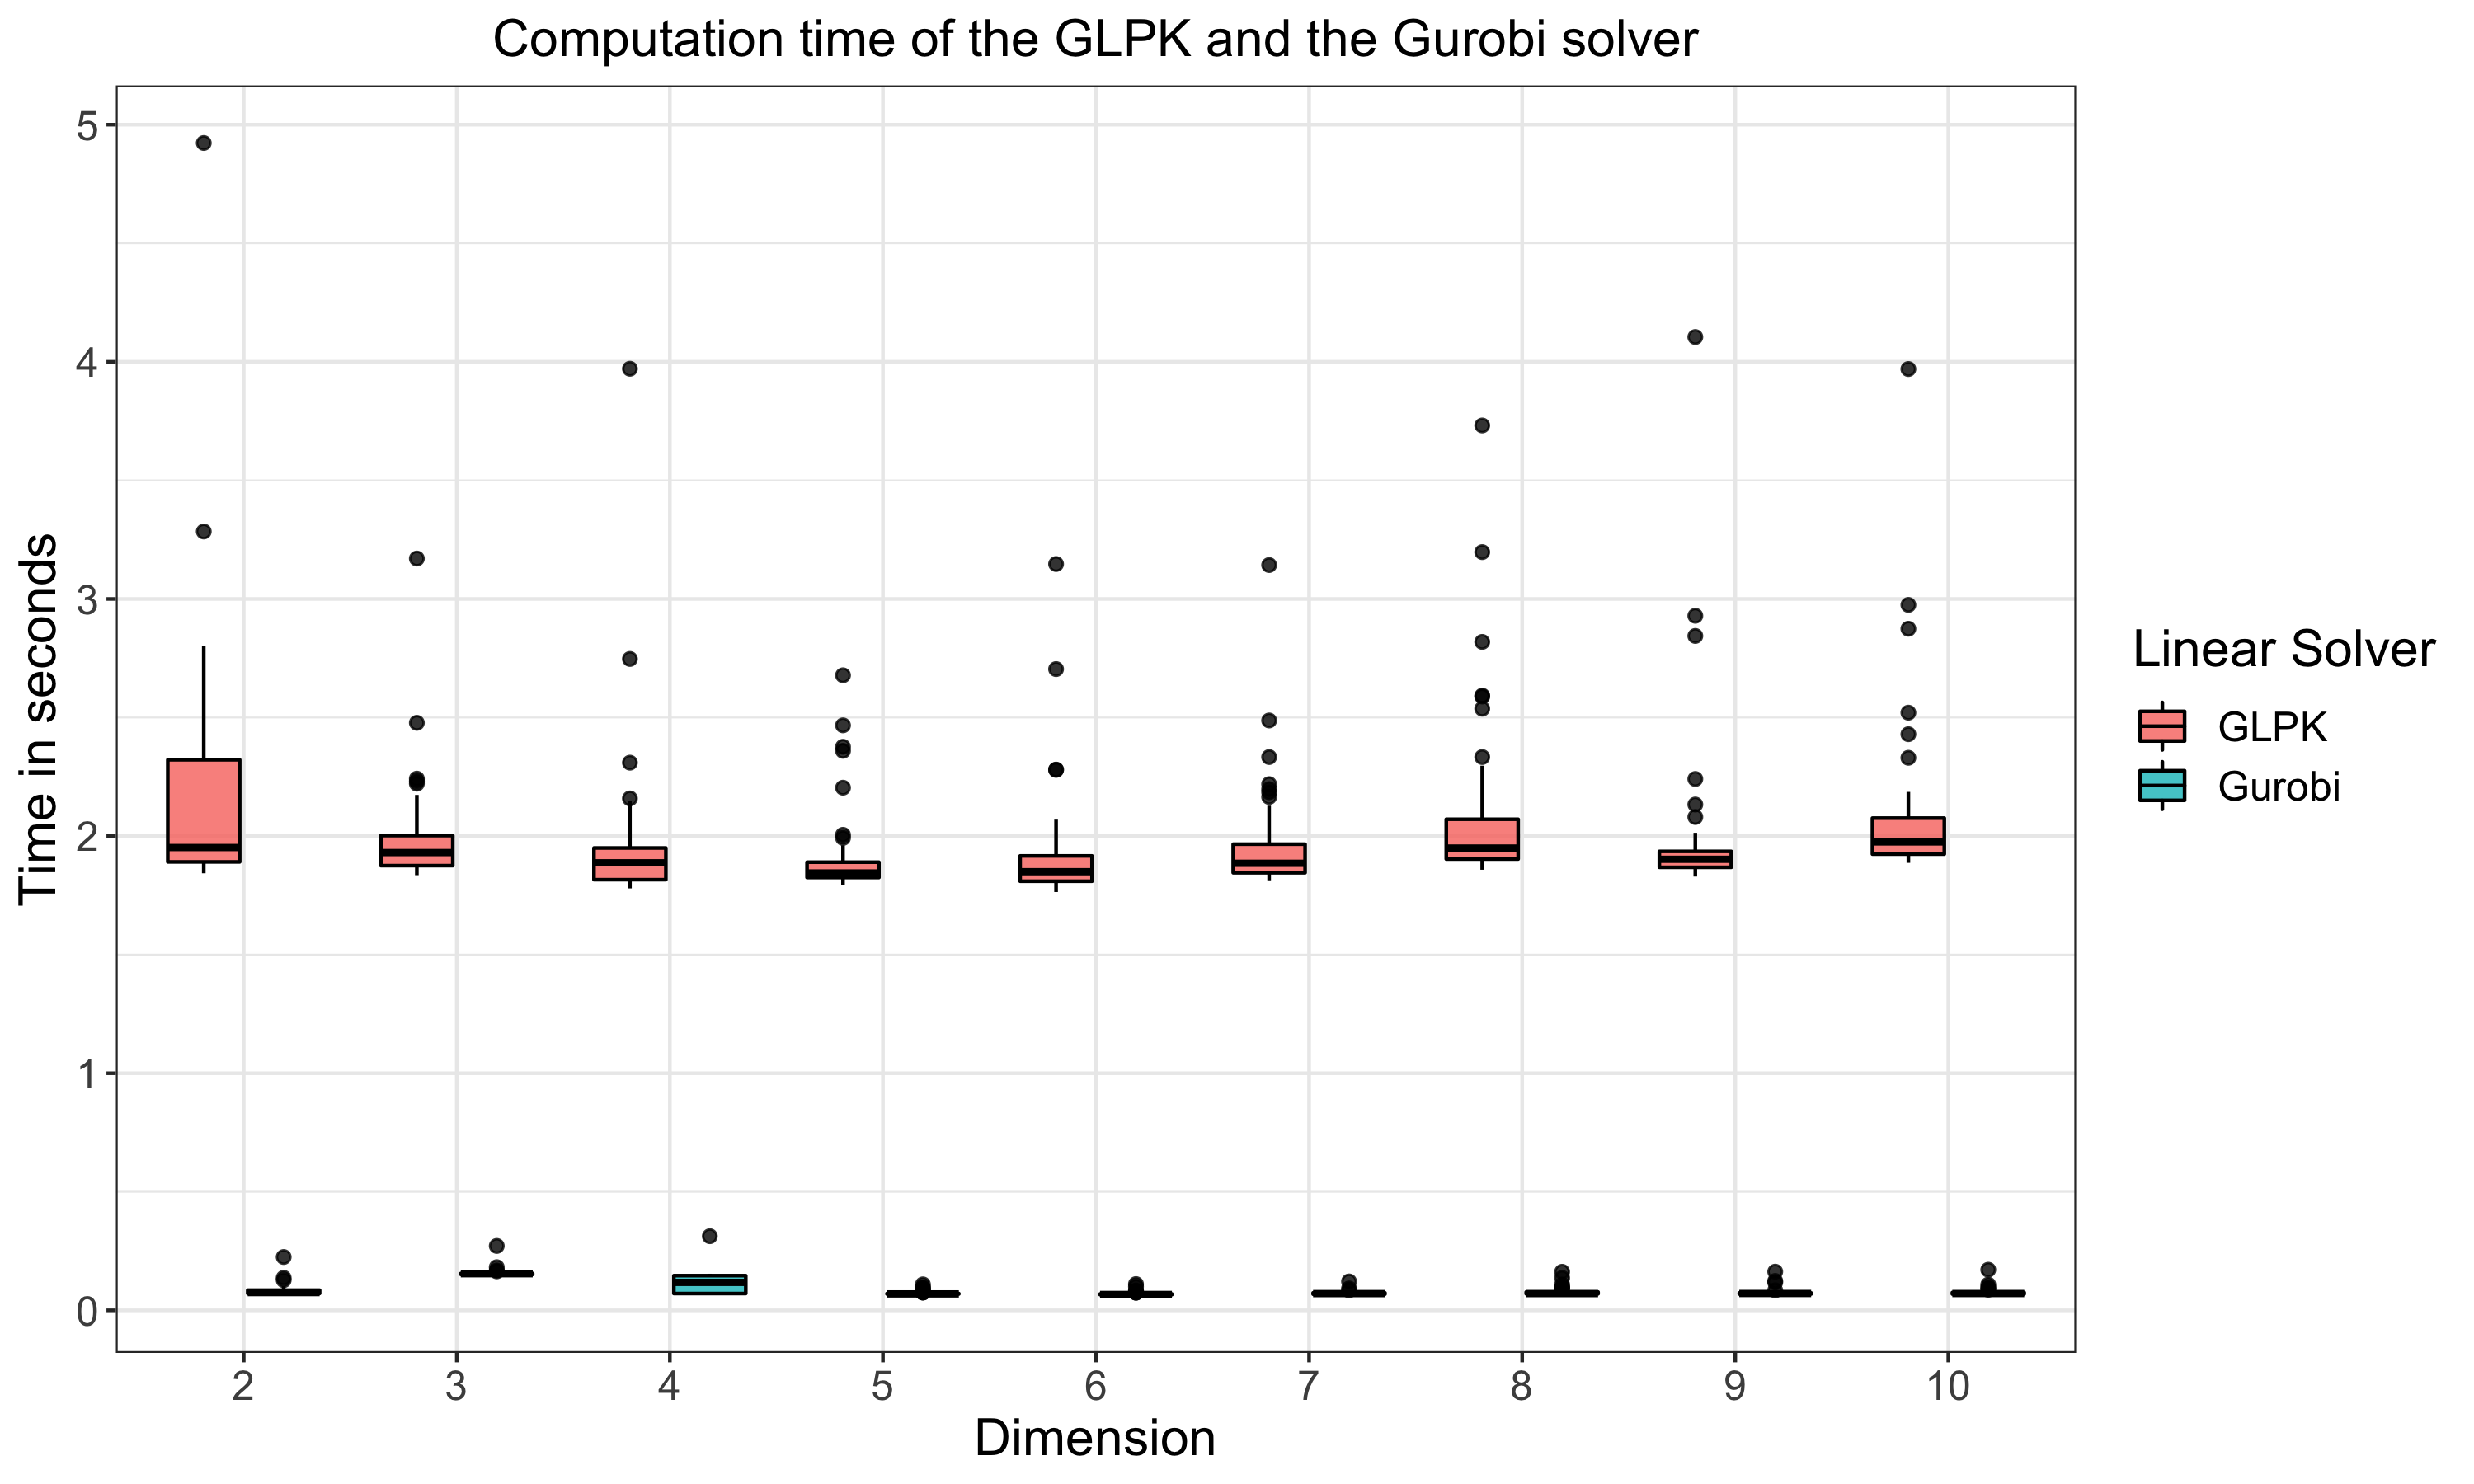
\includegraphics[width=\linewidth, height=2.2in] {graphs/boxplots_glpk_gurobi.png}
    \caption{Computation time of the GLPK and the Gurobi solver}
    \label{comptime}
\end{minipage}
\hfill
\begin{minipage}[b]{3in}
    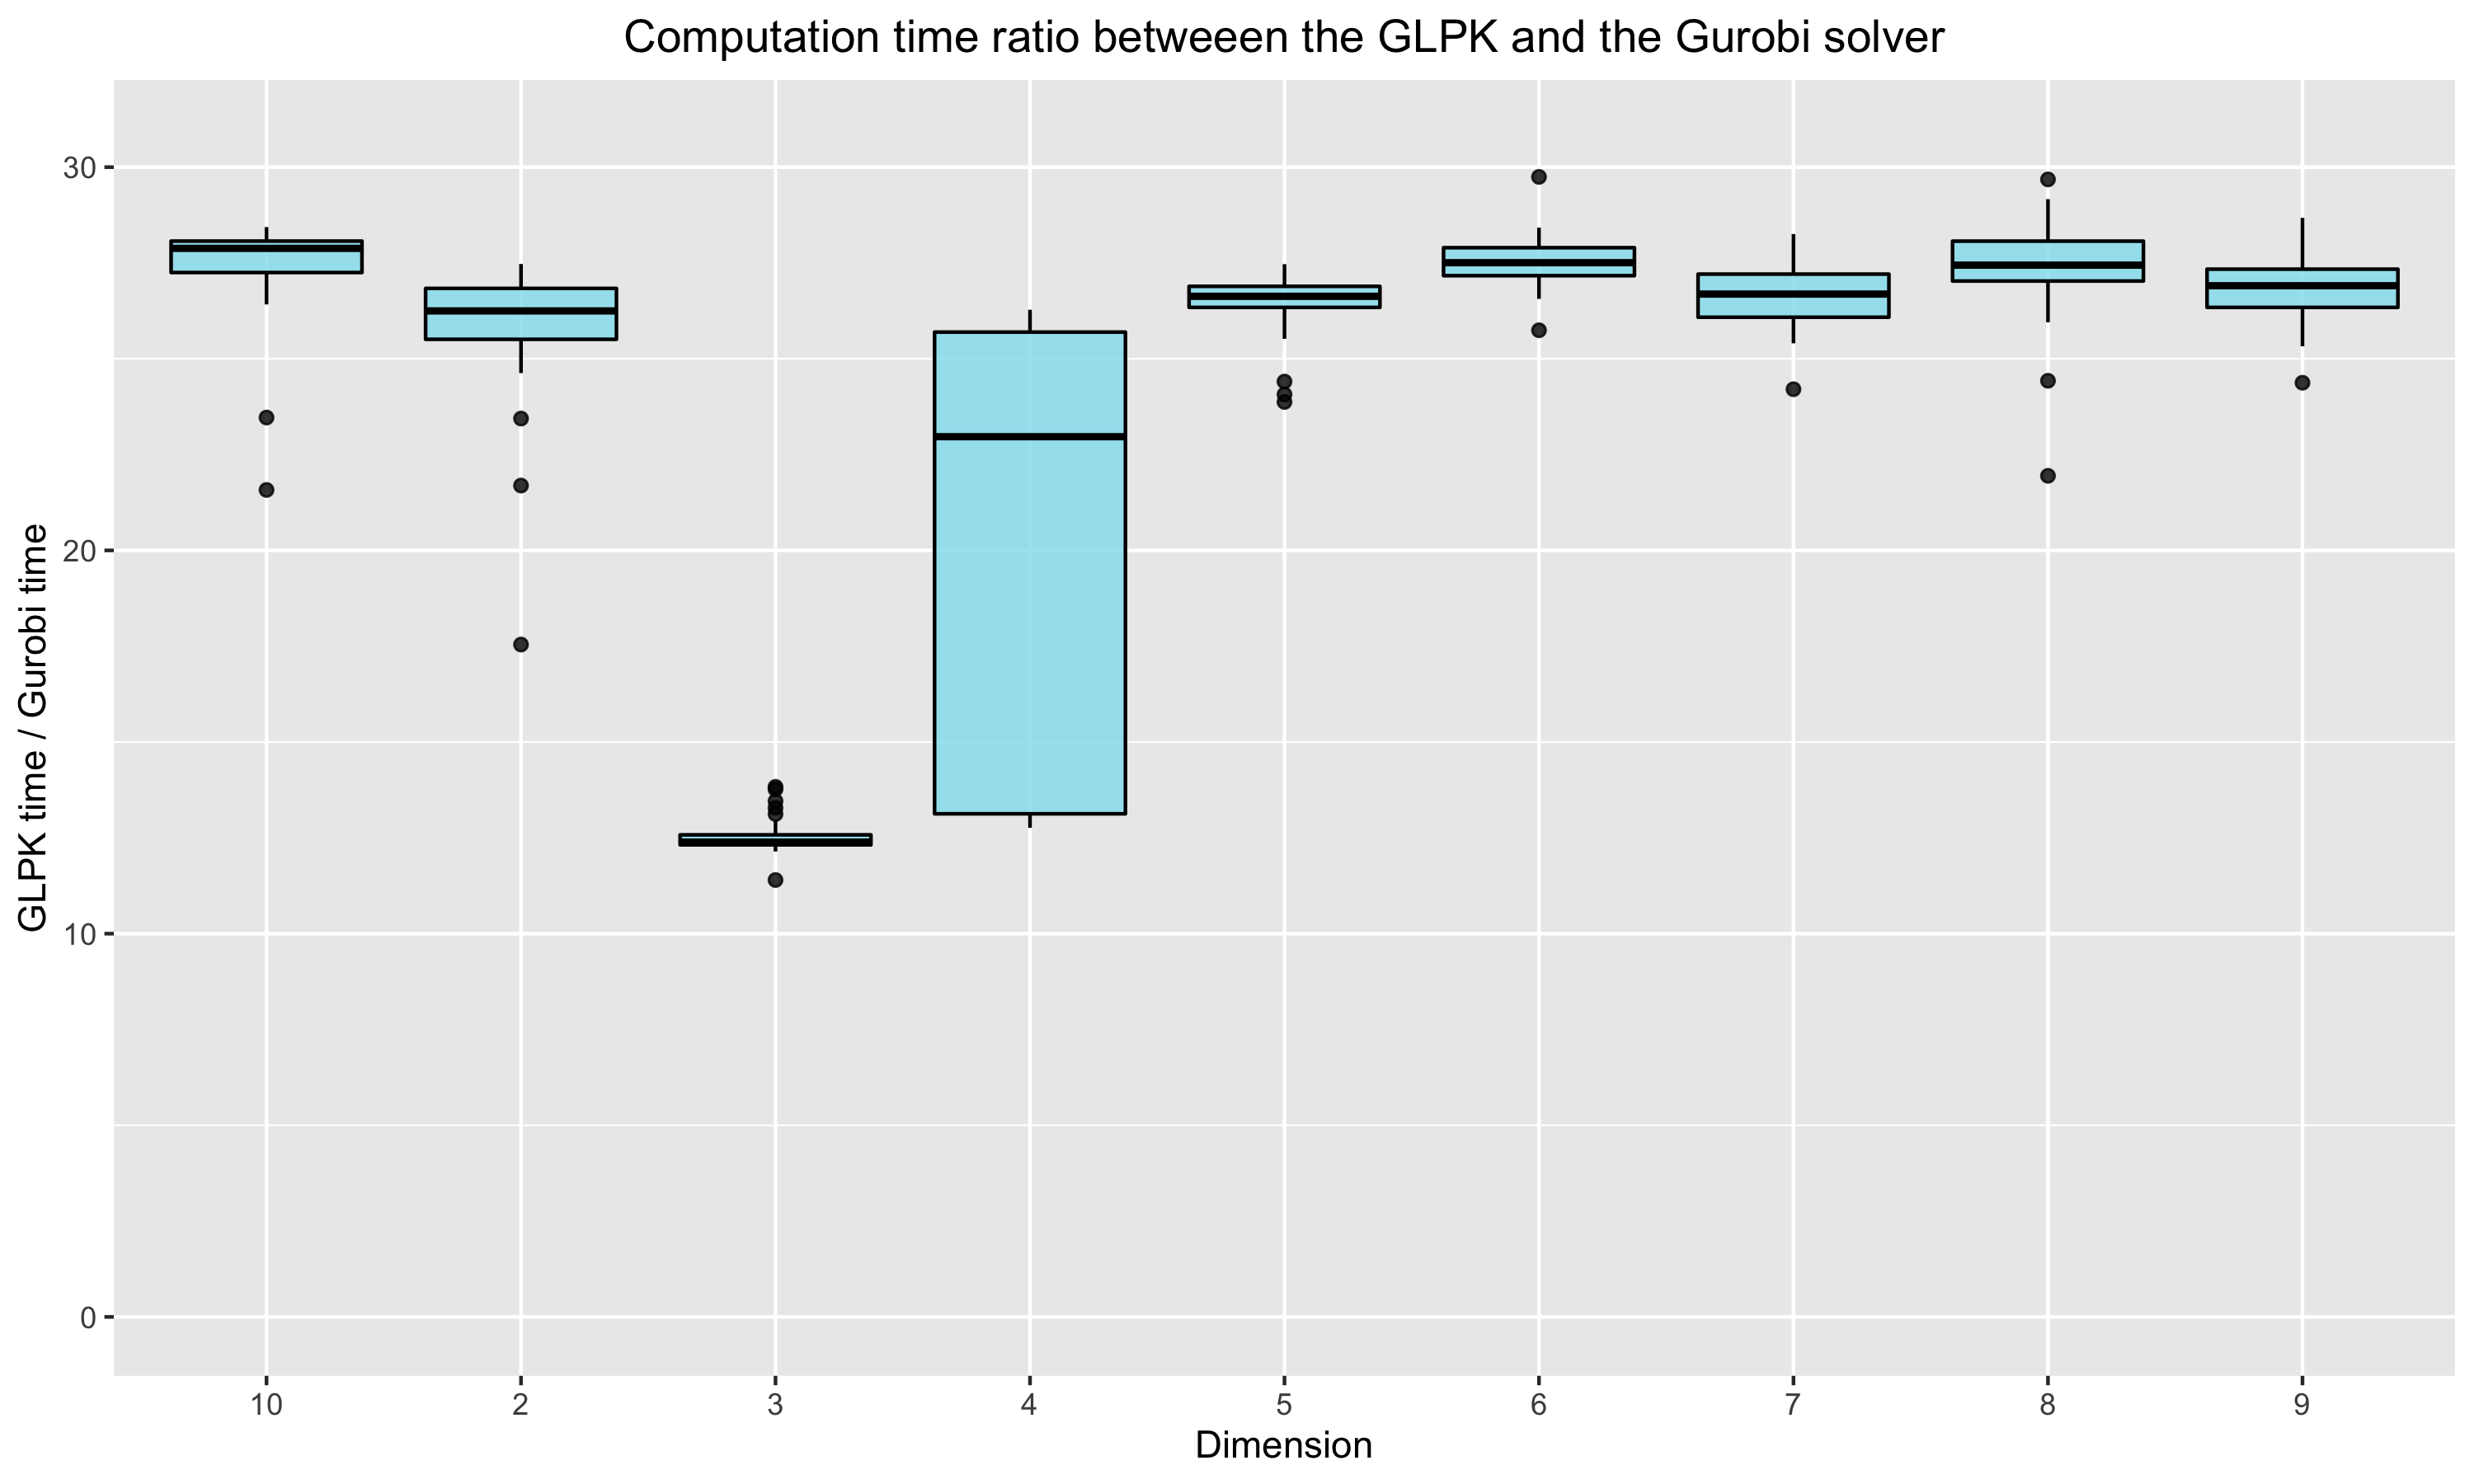
\includegraphics[width=\linewidth, height=2.2in]{graphs/computationratio_glpk_gurobi.png}
    \caption{Computation time ratio between the GLPK and the Gurobi solver}
    \label{compratio}
\end{minipage}
\end{figure}

We compared the performance of the GLPK solver and the Gurobi solver on data sets drawn from the Cauchy distribution. As shown in Figure \ref{comptime} and Figure \ref{compratio}, the average computation time of the GLPK solver is roughly $25$ times the computation time of the Gurobi solver. 


In addition, when not requiring integral solutions, the GLPK solver returned a number of solutions with non-integral entries whereas the Gurobi solver returned all integral  solutions.  In the cases where the GLPK solver did not return an integral solution, the one norm difference between $X^{I}$ and $X^{NI}$ is on the scale of $10^{-16}$, values close to machine $\epsilon$. 

\begin{table}[!h]
    \centering
\begin{tabular}{
|p{2.3cm}||p{2cm}|p{2cm}|p{2cm}|p{2cm}|}
 \hline
 Entry Type & $\x^I_{Len}$ & $\x^{NI}_{Len}$ & $\x^I_{Unif}$ & $\x^{NI}_{Unif}$\\
 \hline
 Integral  & $100\%$    &$98.68\%$&   $100\%$ & $99.47\%$\\
 In $\{-1,0,1\}$&   $100\%$  & $98.68\%$   &$100\%$ & $99.47\%$\\
 Non-Integral & $0\%$ & $1.32\%$&  $0\%$ & $0.53\%$ \\
 \hline
\end{tabular}
\end{table}


For both solvers, the computation time it takes to find an integral solution is in general similar to the computation time it takes to find a non-integral solution. 

\subsection{Benchmark}
We use the Julia package \textit{BenchmarkTools} to measure the performance of each algorithms. 

According to the official documentation, 
the minimum is a robust estimator for the location parameter of the time distribution, and should not be considered an outlier.
The median, as a robust measure of central tendency, should be relatively unaffected by outliers.
The mean, as a non-robust measure of central tendency, will usually be positively skewed by outliers.
The maximum should be considered a primarily noise-driven outlier, and can change drastically between benchmark trials.

\section{Notations}
We use $\x$ to denote the solution to an optimizing problem. Similarly, $\x^I$ denotes solutions to integer programming problems, and $\x^{NI}$ denotes solutions to linear programming problems. We use $\x_{Len}$ to represent solutions optimal against length-weighted loss functions and $\x_{Unif}$ to represent solutions optimal against uniform-weighted loss functions. 

We use $C$ to denote the cost of an optimization problem. $C^I$ represents the cost we get for an integer programming problem while $C^{NI}$ is the cost we get for an linear programming problem. Similarly, $C_{Len}$ represents the length-weighted cost, and $C_{Unif}$ represents the uniform-weighted cost. 

We use $L$ to denote the loss function for an optimization problem. $L^I$ represents the loss function for an integer linear programming problem and $L^{NI}$ represents the loss function for a linear programming problem.
\section{Results}

First, we look at the entries of the optimal solutions. As shown in Table \ref{tab:entry}, all $\x$ we've found have entries in $\{-1, 0, 1\},$ which implies that they are also solutions to the $\ell^0$-optimization problem. \textcolor{blue}{One thing to note that is when using the GLPK solver, we did get non-integral entries when dropping the constraint that the variables be integral, whereas when using the Gurobi solver, all the $\x$ we get were integral and in $\{-1, 0, 1\}.$ } \textcolor{red}{Non-integral look like machine epsilon and report the frequency. }
\begin{table}[!h]
    \centering
\begin{tabular}{
|p{2.3cm}||p{2cm}|p{2cm}|p{2cm}|p{2cm}|}
 \hline
 Entry Type & $\x^I_{Len}$ & $\x^{NI}_{Len}$ & $\x^I_{Unif}$ & $\x^{NI}_{Unif}$\\
 \hline
 Integral  & $100\%$    &$100\%$&   $100\%$ & $100\%$\\
 In $\{-1,0,1\}$&   $100\%$  & $100\%$   &$100\%$ & $100\%$\\
 Non-Integral & $0\%$ & $0\%$&  $0\%$ & $0\%$ \\
 \hline
\end{tabular}
\caption{Minimal Generator Entry Types}
\label{tab:entry}
\end{table}


Since all the solutions we found were $\ell^0$-optimal, we compared the $\ell_0$-optimal solutions to $\ell_1$-optimal solutions. We found that for all the optimal solutions found, the optimum value for $||\mathbf{w} \cdot \x||$ is the same whether we require variables to be integral or not. 

\textcolor{blue}{In terms of the solutions $\x$, we found that $78.78\%$ of the uniform-weighted optimal solutions are identical whether we require the variables to be integral or not and all the length-weighted optimal solutions are identical. This makes sense since with the uniform-weighted loss function, we are minimizing the number of simplices in a generator. Therefore, there might be multiple ways to achieve the optimum whereas with the length-weighted loss function, we are minimizing the total length of the generator. Since almost all simplices have different lengths, it is likely that there is a unique solution to achieve the optimum, though not guaranteed. or: since all simplices have diff length/diameters, it is possible that solutions in this regime are unique. }

\begin{table}[h]
    \centering
    \begin{tabular}{|c|c|c|}
    \hline
         & $\x_{Unif}$ & $\x_{Len}$\\ \hline
         $C^{I} = C^{NI}$ & $100\%$  & $100\%$ \\ \hline
         $X^I = X^{NI}$ & $80.29\%$ & $100\%$ \\ \hline
    \end{tabular}
    \caption{$\ell_1$ solutions and $\ell_0$ solutions}
    \label{tab:my_label}
\end{table}
Then, we examine the effectiveness of the uniform-weighted and length-weighted optimal solutions. In Table \ref{tab:effectiveness}, we calculated the average ratio of the loss between different optimal solutions found. \textcolor{blue}{ Since all the optimal solutions achieve the same optimum value whether requring integer or not, we have the same values for $\x^{I}$ and $\x^{NI}$ columns. }

\begin{table}[H]
    \centering
    \begin{tabular}{|c|c|c|}
    \hline
         & $\x^{I}$ & $\x^{NI}$\\ \hline
         $  \overline{\frac{L_{Len}(X_{Len})}{L_{Len}(X_{Original})}}$ & $69.36\%$  & $69.36\%$ \\ \hline
         $\overline{\frac{L_{Unif}(X_{Unif})}{L_{Unif}(X_{Original})}}$ & $67.49\%$ & $67.49\%$ \\ \hline
    \end{tabular}
    \caption{ Average ratio between loss of minimal generators and loss of the original generator }
    \label{tab:effectiveness}
\end{table}
\footnote{Note: entries of this table are the average ratio between different loss functions of different optimal solutions.}

\begin{figure}[H]
  \centering
  \begin{minipage}[b]{0.45\textwidth}
    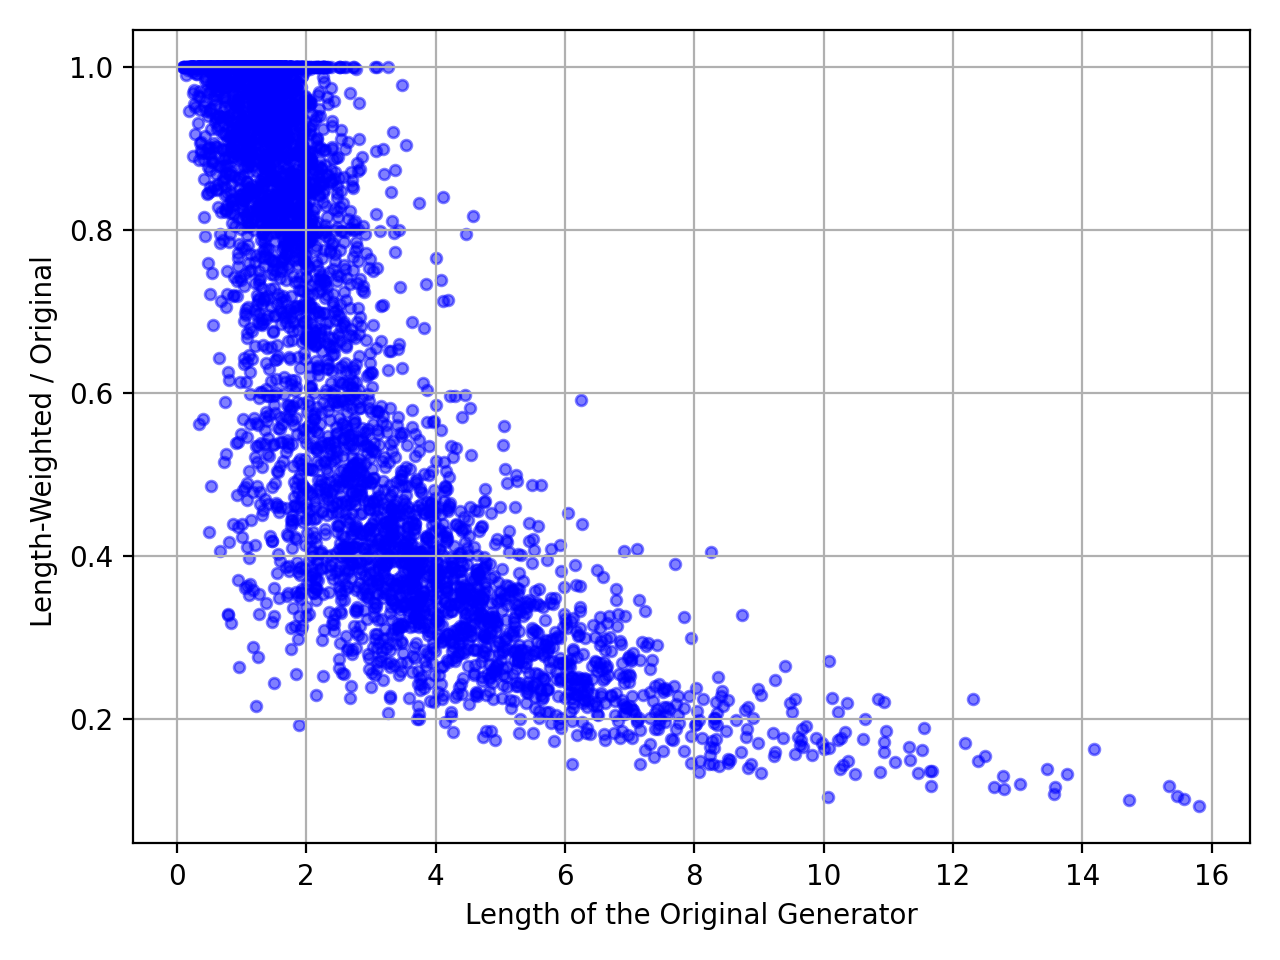
\includegraphics[width=\textwidth]{graphs/len_eff.png}
    \caption{Length-Weighted Minimal Generators}
  \end{minipage}
  \hfill
  \begin{minipage}[b]{0.45\textwidth}
    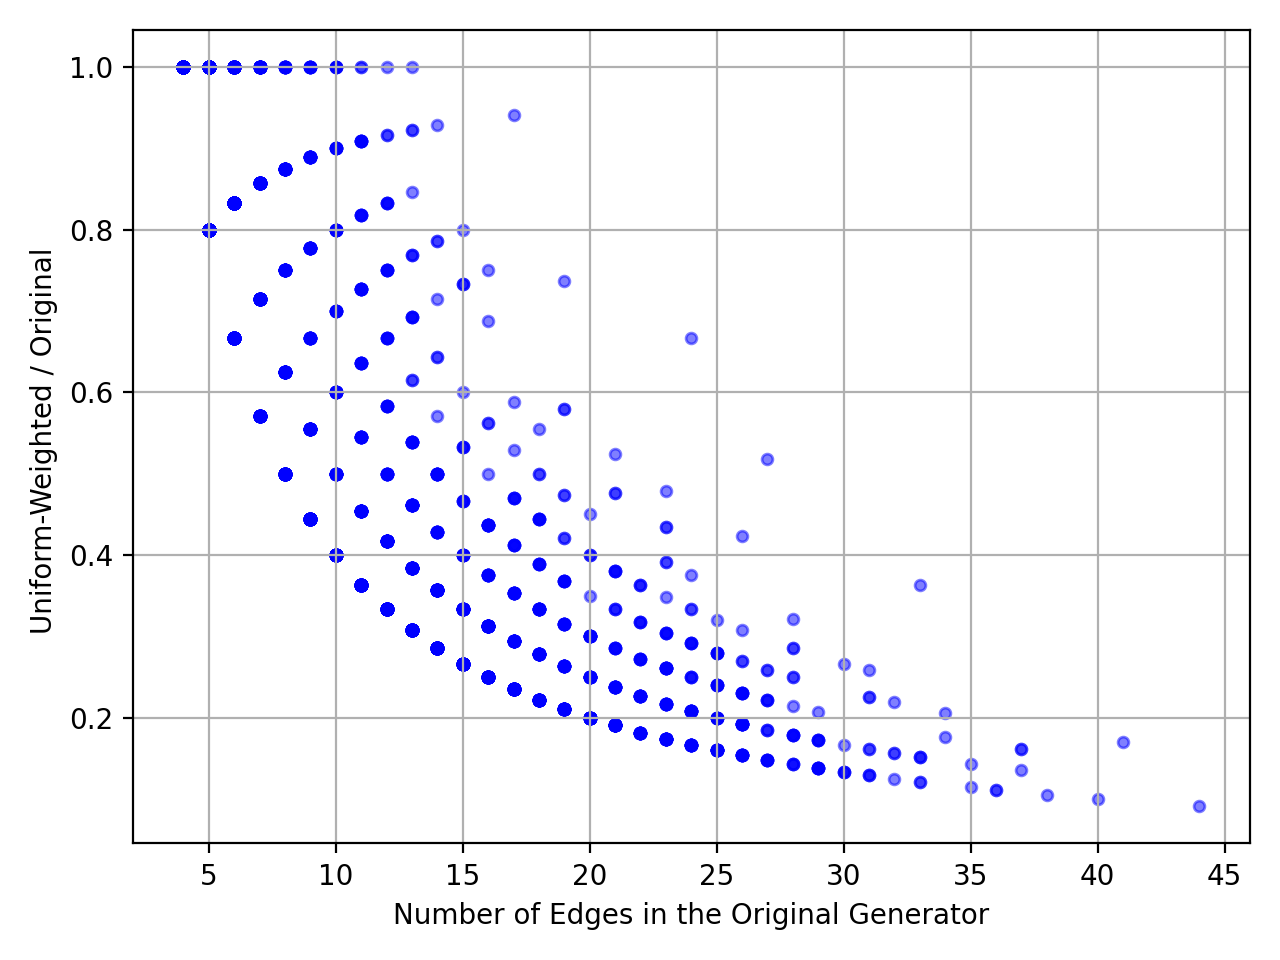
\includegraphics[width=\textwidth]{graphs/unif_orig_int.png}
    \caption{Uniform-Weighted Minimal Generators}
  \end{minipage}
\end{figure}

In addition to examining the optimal solutions of two different weighted loss functions against the original generators, we also evaluate the optimal solutions  found under one loss function against the other loss function. 

\begin{table}[H]
    \centering
    \begin{tabular}{|c|c|c|}
    \hline
         & $\x^I$ & $\x^{NI}$ \\ \hline
         $L_{Len}(\x_{Unif}) = L_{Len}(\x_{Len})$ & $63.46\%$  & $63.82\%$ \\ \hline
         $L_{Unif}(\x_{Len}) = L_{Unif}(\x_{Unif})$ & $99.81\%$ & $99.81\%$ \\ \hline
    \end{tabular}
    \caption{Evaluating $\ell_1$ and $\ell_0$ solutions against the other loss function}
    \label{table:optimalboth}
\end{table}
Explain why first row not equal across
Look into second row some length minimal does not have minimal edges 

From table \ref{table:optimalboth}, we can see that the optimal solutions we get when optimizing against the length-weighted loss functions are also typically optimal against the uniform-weighted loss function, but not vice versa. \textcolor{blue}{We report the mean and standard deviation for the distribution of the difference in cost values for non-integer solutions in Table \ref{table:stats}.}

\begin{table}[H]
    \centering
    \begin{tabular}{|c|c|c|}
    \hline
         & mean & standard deviation \\ \hline
         $|L_{Len}(\x_{Unif}) - L_{Len}(\x_{Len})|$ & $0.022805$  & $0.044352$ \\ \hline
         $|L_{Unif}(\x_{Len}) - L_{Unif}(\x_{Unif})|$ & $0.002367$ & $0.048601$ \\ \hline
    \end{tabular}
    \caption{Evaluating $\ell_1$ and $\ell_0$ solutions against the other loss function}
    \label{table:stats}
\end{table}



Then, we compare the computation time our programs took to solve the integer linear programming and non integeral programming optimization problems. On average, the median computation time an integer linear programming takes is $1.15$ times the median computation time an linear programming takes.  

\begin{figure}[!h]
  \centering
  \begin{minipage}[b]{0.45\textwidth}
    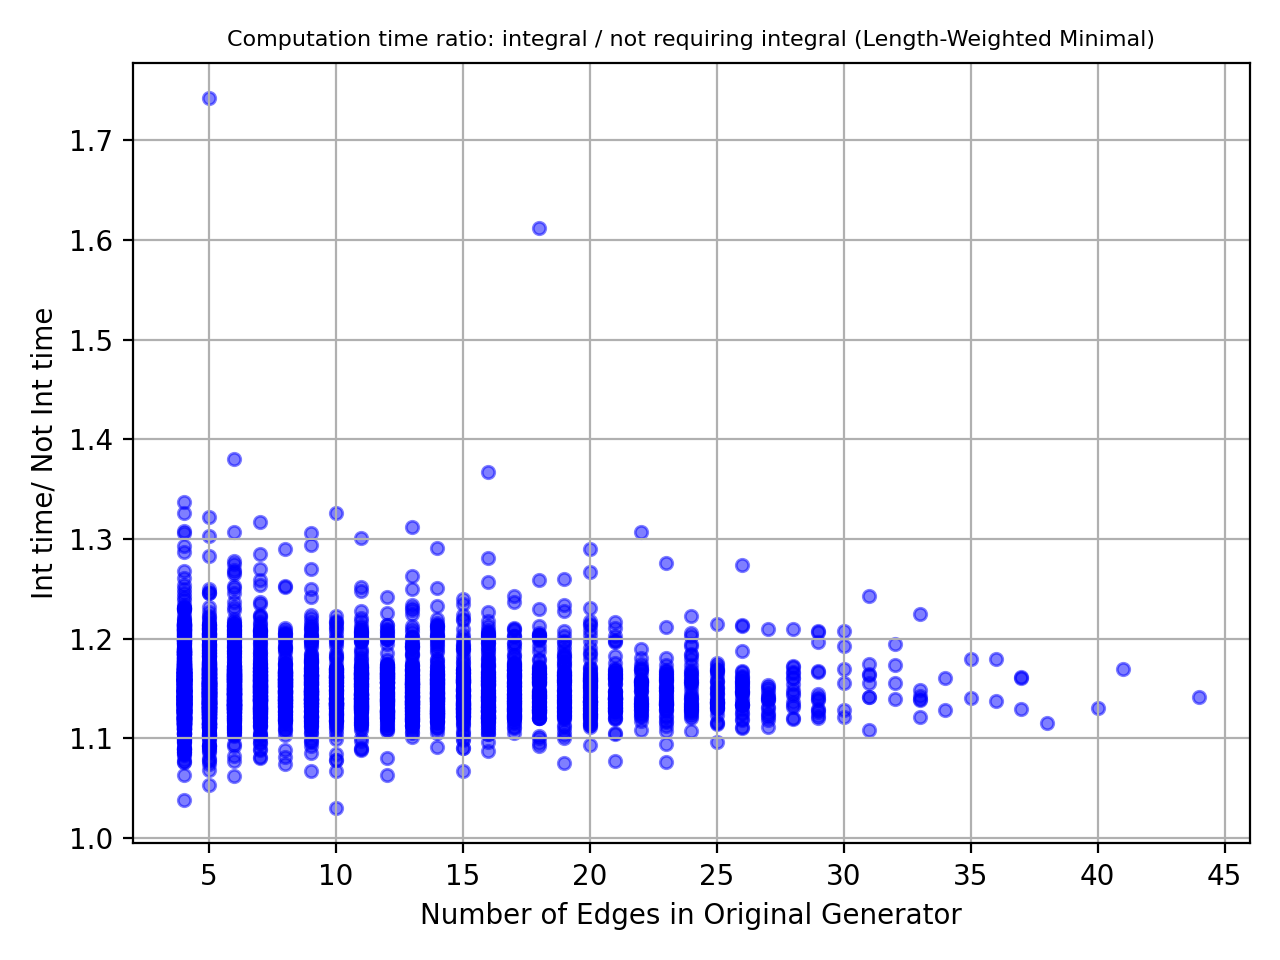
\includegraphics[width=\textwidth]{graphs/len_time_ratio.png}
    \caption{Length-Weighted Minimal Generators}
  \end{minipage}
  \hfill
  \begin{minipage}[b]{0.45\textwidth}
    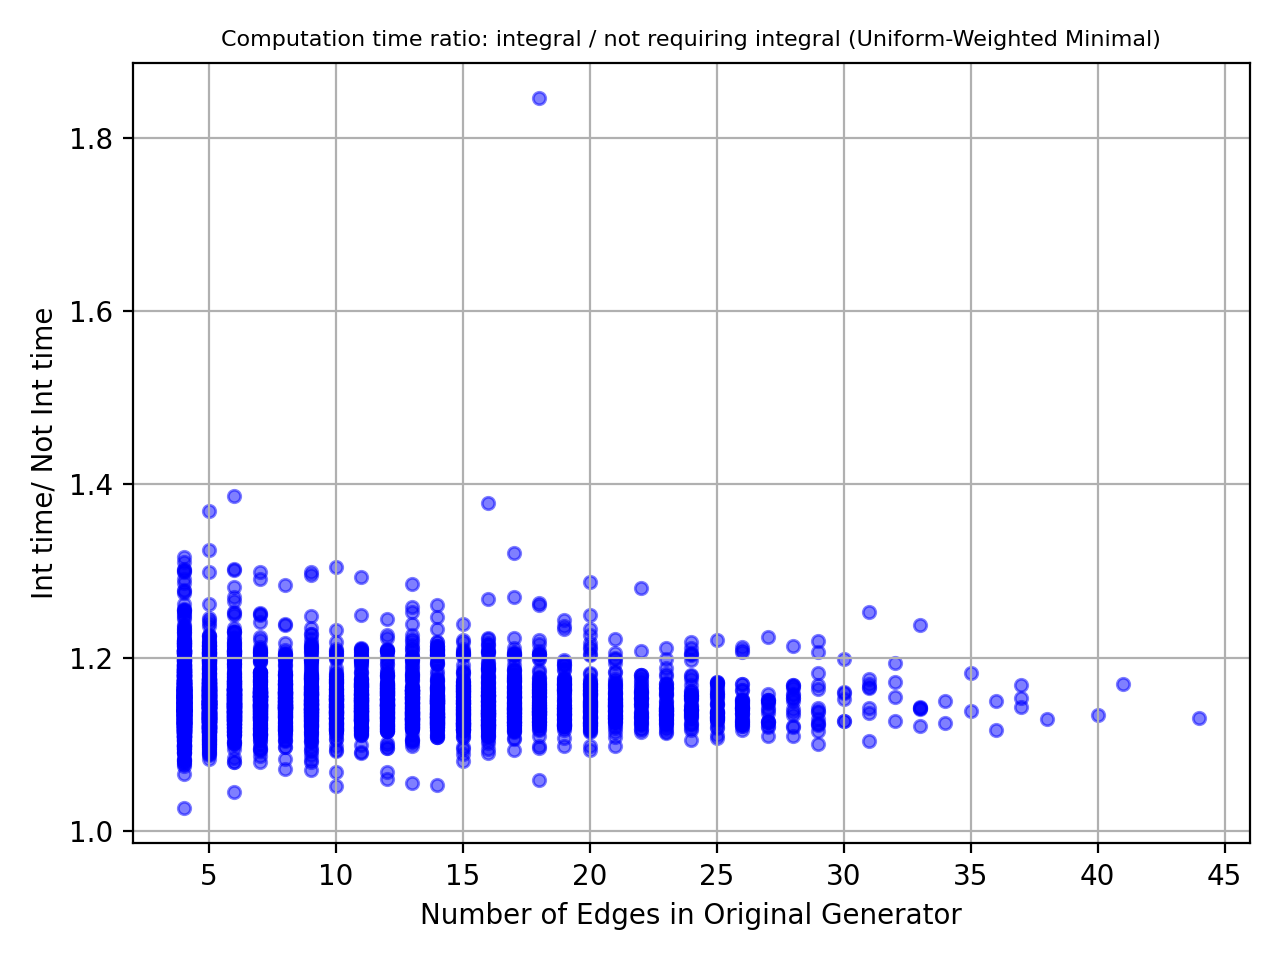
\includegraphics[width=\textwidth]{graphs/unif_time_ratio.png}
    \caption{Uniform-Weighted Minimal Generators}
  \end{minipage}
\end{figure}

\begin{table}[h]
    \begin{tabular}{|c|c|c|}
    \hline
         & Length-Weighted Minimal Generator & Uniform-Weighted Minimal Generator\\ \hline
         $\overline{Time^{I} / Time^{NI}}$ & $1.15$  & $1.15$ \\ \hline
    \end{tabular}
    \caption{Average Time Ratio of $L_0$ solutions and $L_1$ solutions}
    \label{tab:my_label}
\end{table}

Below is a plot which summarizes the generator size of each distribution in each dimension. 

\begin{figure}[h]
    \centering
    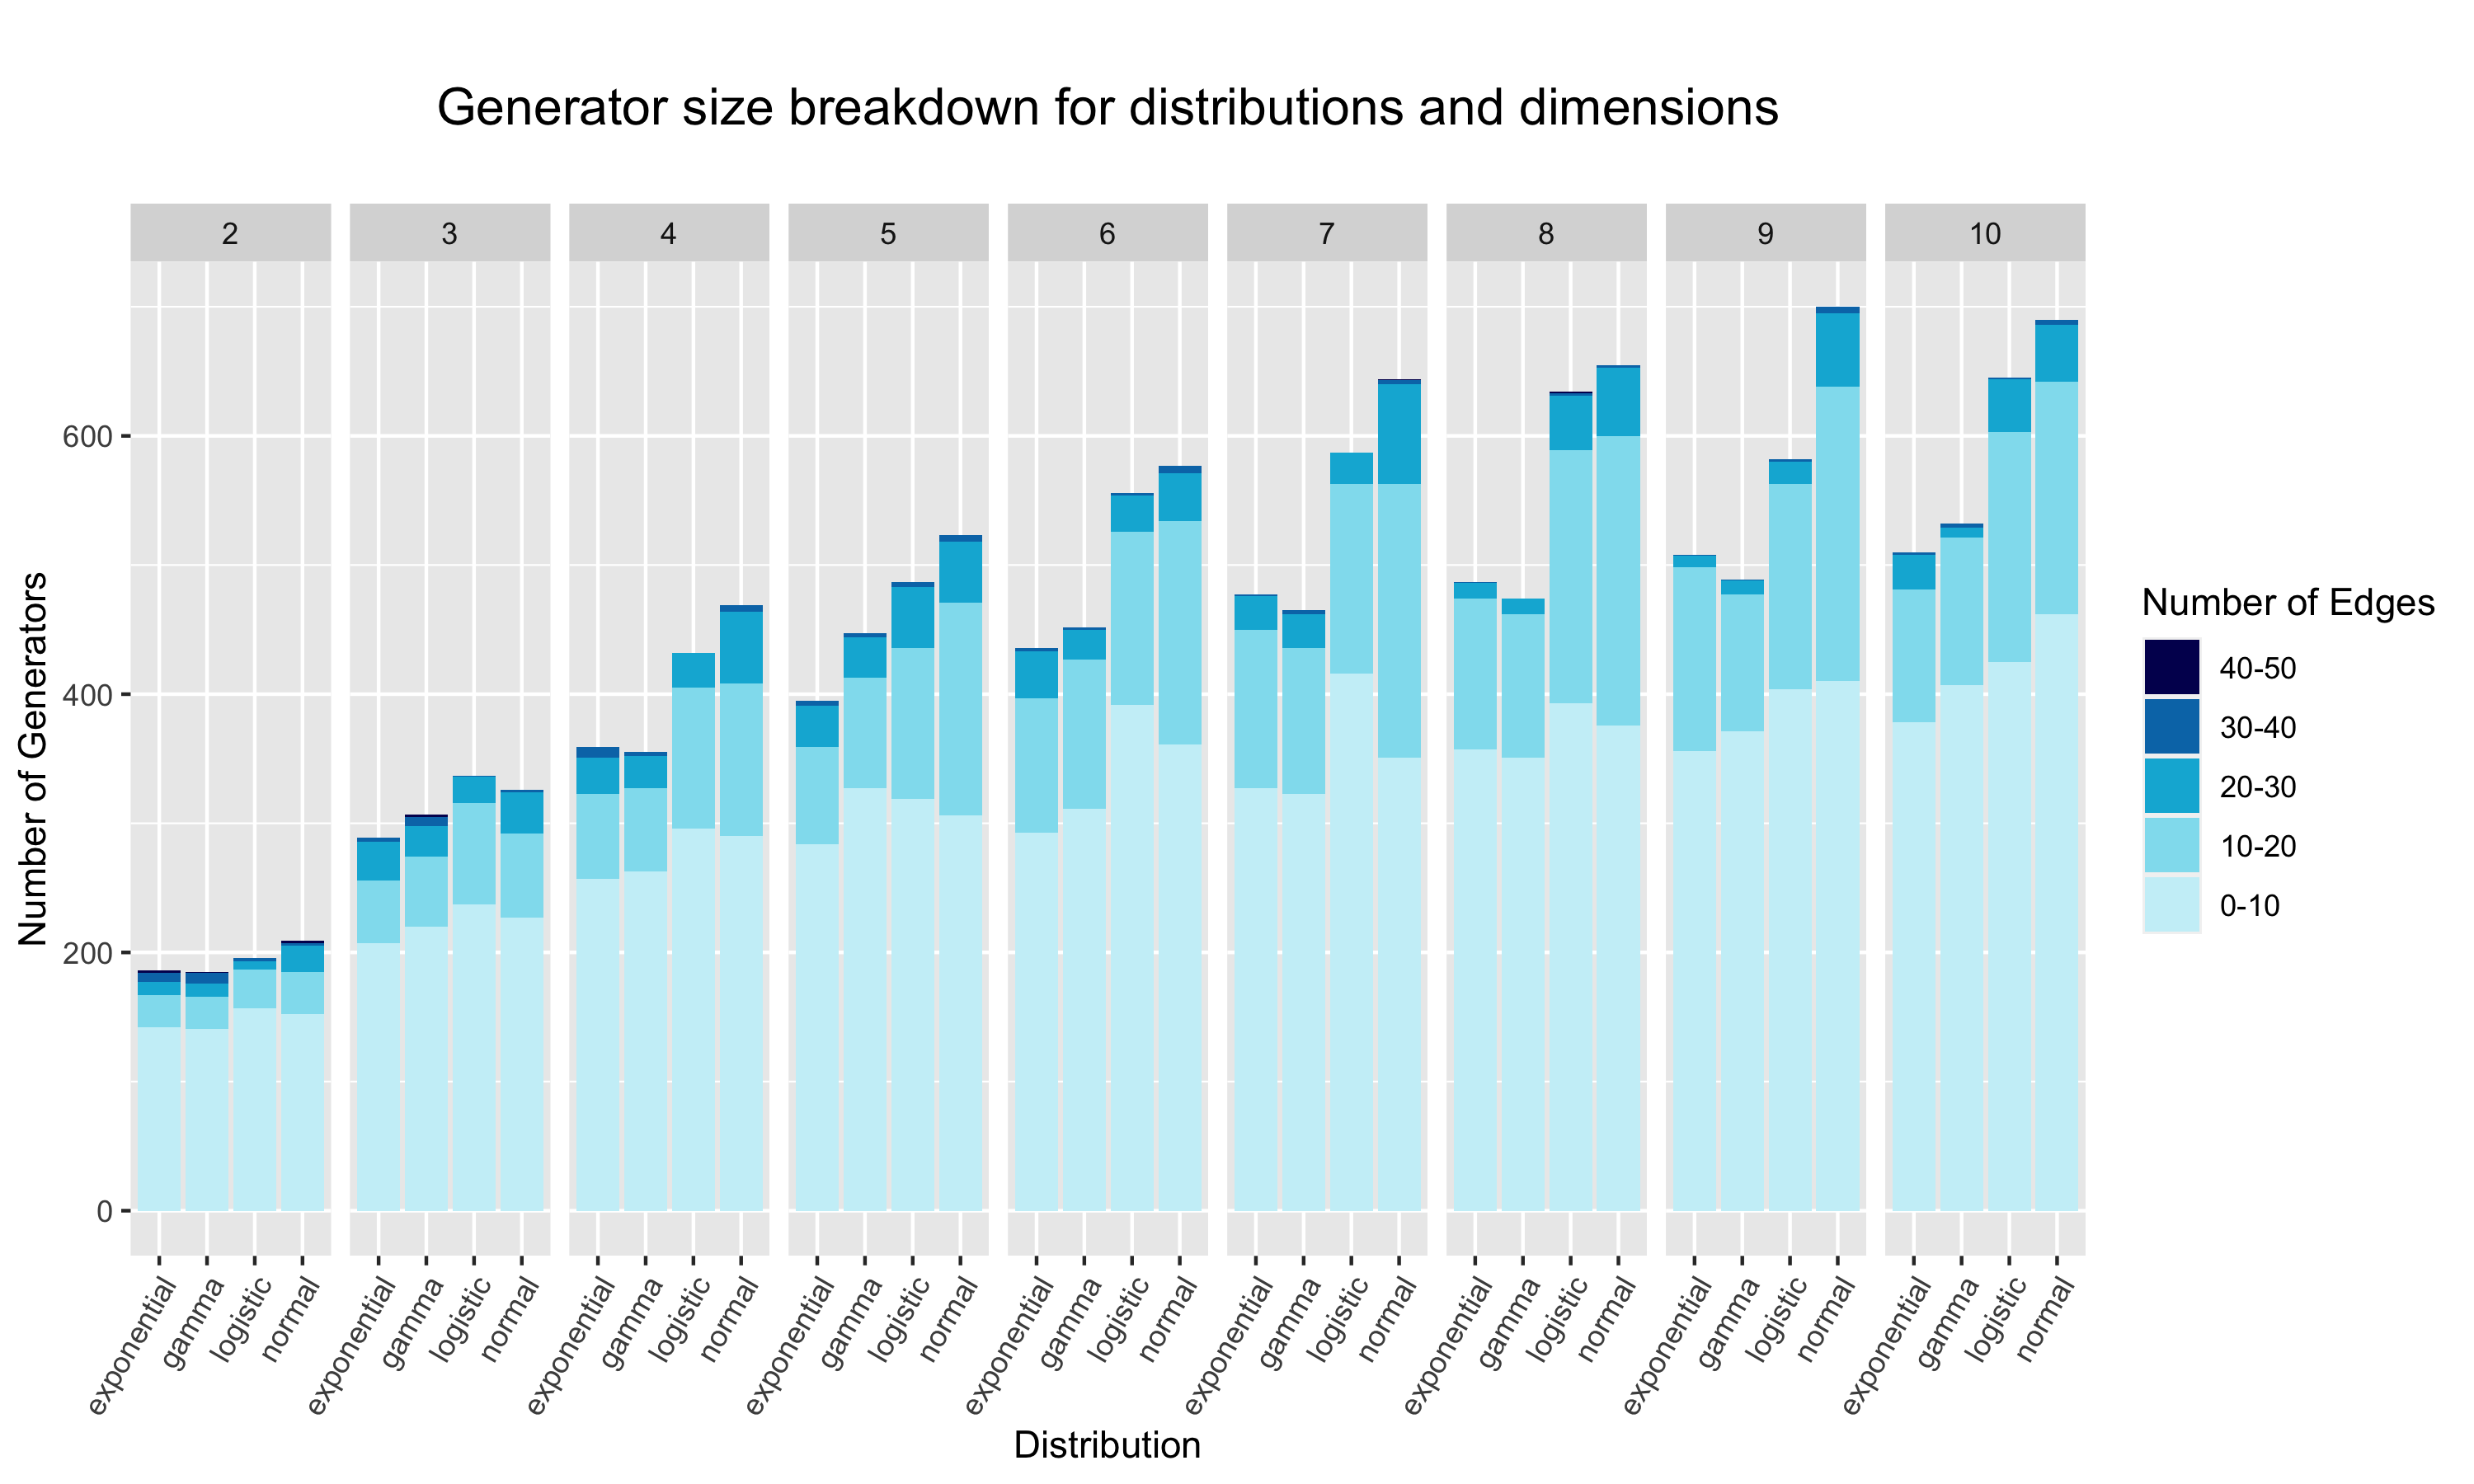
\includegraphics[width=6in]{graphs/generator_numbers.png}
    \caption{Generators numbers and size breakdown for different distributions and dimensions}
    \label{fig:my_label}
\end{figure}

We also examine the relationship between the computation time with the size of the boundary matrix in the optimization problem. As shown in Figure \ref{fig:lm}, there is a linear relationship

\begin{figure}[h]
    \centering
    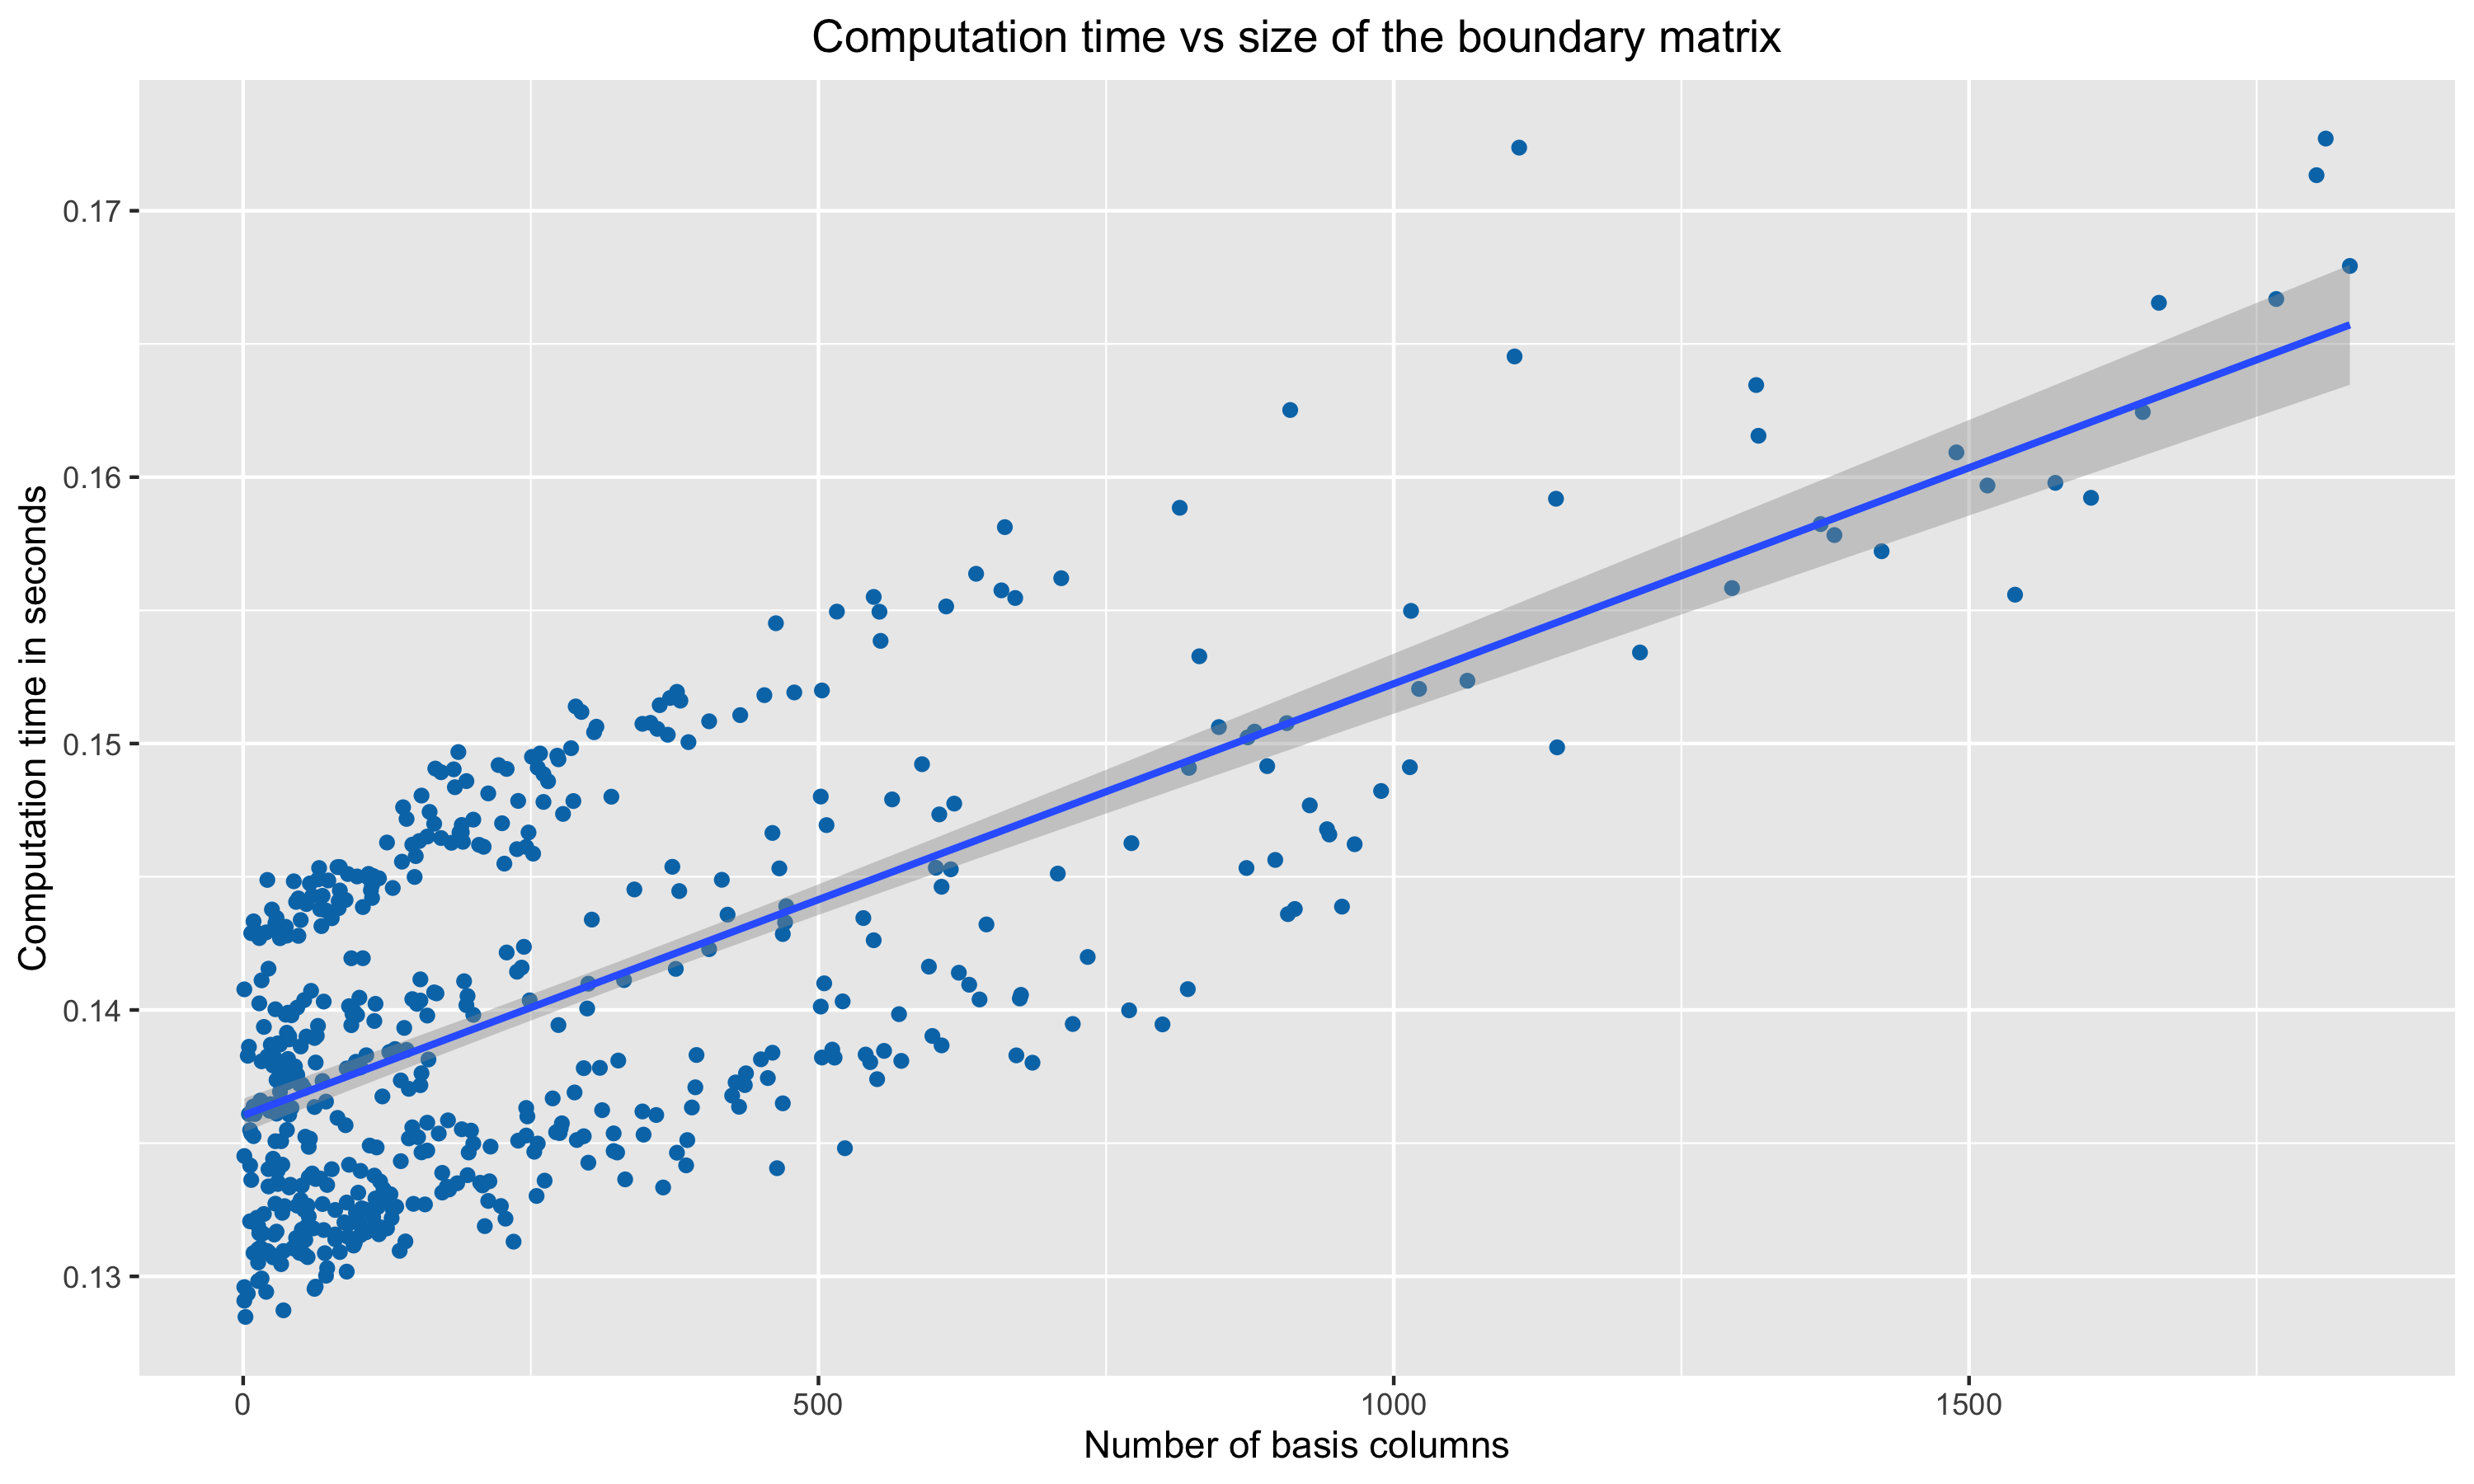
\includegraphics[width=5in]{graphs/time_sizebdrmatrix.png}
    \caption{Relationship between computation time and boundary matrix size}
    \label{fig:lm}
\end{figure}

\newpage
\section{Conclusions}

\bibliographystyle{alpha}
\bibliography{biblio}


\end{document}
